\chapter{Pilastro}\label{chap:pilastro}
Come descritto nel capitolo~\ref{sec:azioniPilastri} il pilastro più sollecitato risulta essere il $P27$. L'azione assiame di compressione massima si sviluppa alla base del pilastro e vale - in combinazione agli stati limite ultimi
\begin{equation}
    \label{eq:NEd_slu}
	N_{Ed} \simeq 1882\,kN
\end{equation}

\section{Progetto e verifica agli SLU}
Il progetto della sezione di calcestruzzo e del quantitativo di armatura presente nel pilastro viene eseguito seguendo quanto riportato al punto \textbf{4.1.6.1.2} delle \textbf{NTC 2018}. Per quanto riguarda l'area delle armature, la normativa italiana assume che il $10\%$ dell'azione assiale di progetto deve essere assorbita dalle armature; cioè
\begin{equation}
    \label{eq:Asmin}
	A_{s,min} = 0.10\,\dfrac{N_{Ed}}{f_{yd}} = 0.10\,\dfrac{1882\cdot 10^3\,N}{391.30\,MPa} = 480.96\,mm^2
\end{equation}

Il calcestruzzo, perciò, dovrà assorbire la restante aliquota
\begin{equation}
    \label{Acmin}
	A_{c,min} = 0.9\,\dfrac{N_{Ed}}{f_{cd}} = 119534.227\,mm^2
\end{equation}
ed assumendo la sezione del pilastro quadrata, il valore minimo del lato è di 
\begin{equation}
    \label{eq:lmin}
	b_{min} = \sqrt{A_{c,min}} = 345.74\,mm
\end{equation}

Si sceglie un valore di lato della sezione in calcestruzzo pari a 
\begin{align}
    \label{eq:l}
	b &= h = 350\,mm\\
	A_c &= b\cdot h = (350\,mm)^2 = 122500\,mm^2	
\end{align}

La normativa fissa dei valori minimi e massimi di armatura pari a 
\begin{align*}
	A_{s,min} &= 480.96\,mm^2 > 0.003\,A_c = 367.50\,mm^2\\
	A_{s,max} &= 0.04\,A_c = 4900\,mm^2
\end{align*}
e comunque non meno di quattro barre (una per spigolo). Il diametro minimo imposto dalle \ntc è di $12\,mm$, da cui si può ricavare un altro limite di area minima che vale
\[
A_{s, min} = 4\,\Phi\,12\,mm = 4\cdot\pi\cdot\dfrac{4^2}{4} = 144\,\pi\,mm^2 = 452.389\,mm^2
\]

L'interasse massimo ammesso tra le barre longitudinali è limitato a $300\,mm$. Avendo una sezione di lato $l = 350\,mm$ il limite posto sull'interasse sarebbe soddisfatto solamente considerando un adeguato copriferro. Cautelativamente si sceglie di inserire delle barre intermedie, dai cui
\[
A_{s,tot} = 6\,\Phi\,18\,mm = 486\,\pi\,mm^2 = 1526.81\,mm^2
\]

L'armatura trasversale deve essere posizionata con un interasse massimo di
\[
s_{max} = \min\{12\,\Phi_{l,min}; 250\,mm\} = \,\min\{216\,mm; 250\,mm\} = 216\,mm
\]
e con un diametro minimo delle staffe di
\[
\Phi_{st,min} = \max\left\{\dfrac{\Phi_{l,max}}{4}; 6\,mm\right\} = \max\{4.5\,mm; 6\,mm\} = 6\,mm
\]

Si sceglie, arrotondando i valori appena calcolati
\begin{align}
	\label{eq:s_pilastro}
	s &= 210\,mm\\
	\label{eq:Phi_st_pilastro}
	\Phi_{st} &= 8\,mm
\end{align}

Definita la sezione e l'armatura si può calcolare il valore di azione assiale resistente. La \circolare al punto \textbf{C4.1.2.3.4.2} definisce la resistenza all'azione assiale dei pilastri - che tiene conto dell'eccentricità minima dei carichi - come
\begin{equation}
    \label{eq:NRd}
	N_{Rd} = 0.8\cdot A_c\,f_{cd} + A_{s,tot}\,f_{yd} = 1986.10\,kN > N_{Ed} = 1882\,kN
\end{equation}

A causa della non perfetta centralità dei carichi agenti sul pilastro, la normativa richiede una ulteriore verifica a flessione sul pilastro, considerando un'eccentricità pari a 
\[
e = \max\left\{\dfrac{l_0}{200}; 20\,mm\right\}
\]
dove $l_0$ è la lunghezza di libera inflessione del pilastro e dipende dalle condizioni al contorno. Se si considera  $l_0 = l$. Assumendo la struttura come un telaio a nodi fissi si può scegliere - a favore di sicurezza - uno schema statico a doppio appoggio per cui $l_0 = l$, dove per $l$ si sceglie l'altezza di interpiano massima  dell'edificio
\[
e = \max\left\{\dfrac{3500\,mm}{200}; 20\,mm\right\} =\max\left\{17.50; 20\right\}\,mm = 20\,mm
\]
Il momento agente sarà
\[
M_{Ed} = e\cdot N_{Ed} = 20\cdot 10^{-3}\,m \cdot 1882\,kN = 37.64\,kN\,m
\]

La verifica viene effettuata calcolando il momento resistente in funzione dell'azione assiale agente
\[
M_{Rd} = M_{Rd}(N_{Ed}) \geq M_{Ed}
\]

Plottando il dominio di resistenza della sezione appena definita e confrontandolo con le sollecitazioni agenti si riscontra che quest'ultime ricadono all'interno del dominio e perciò la sezione è verificata a flessione. 

\begin{figure}
    \centering
	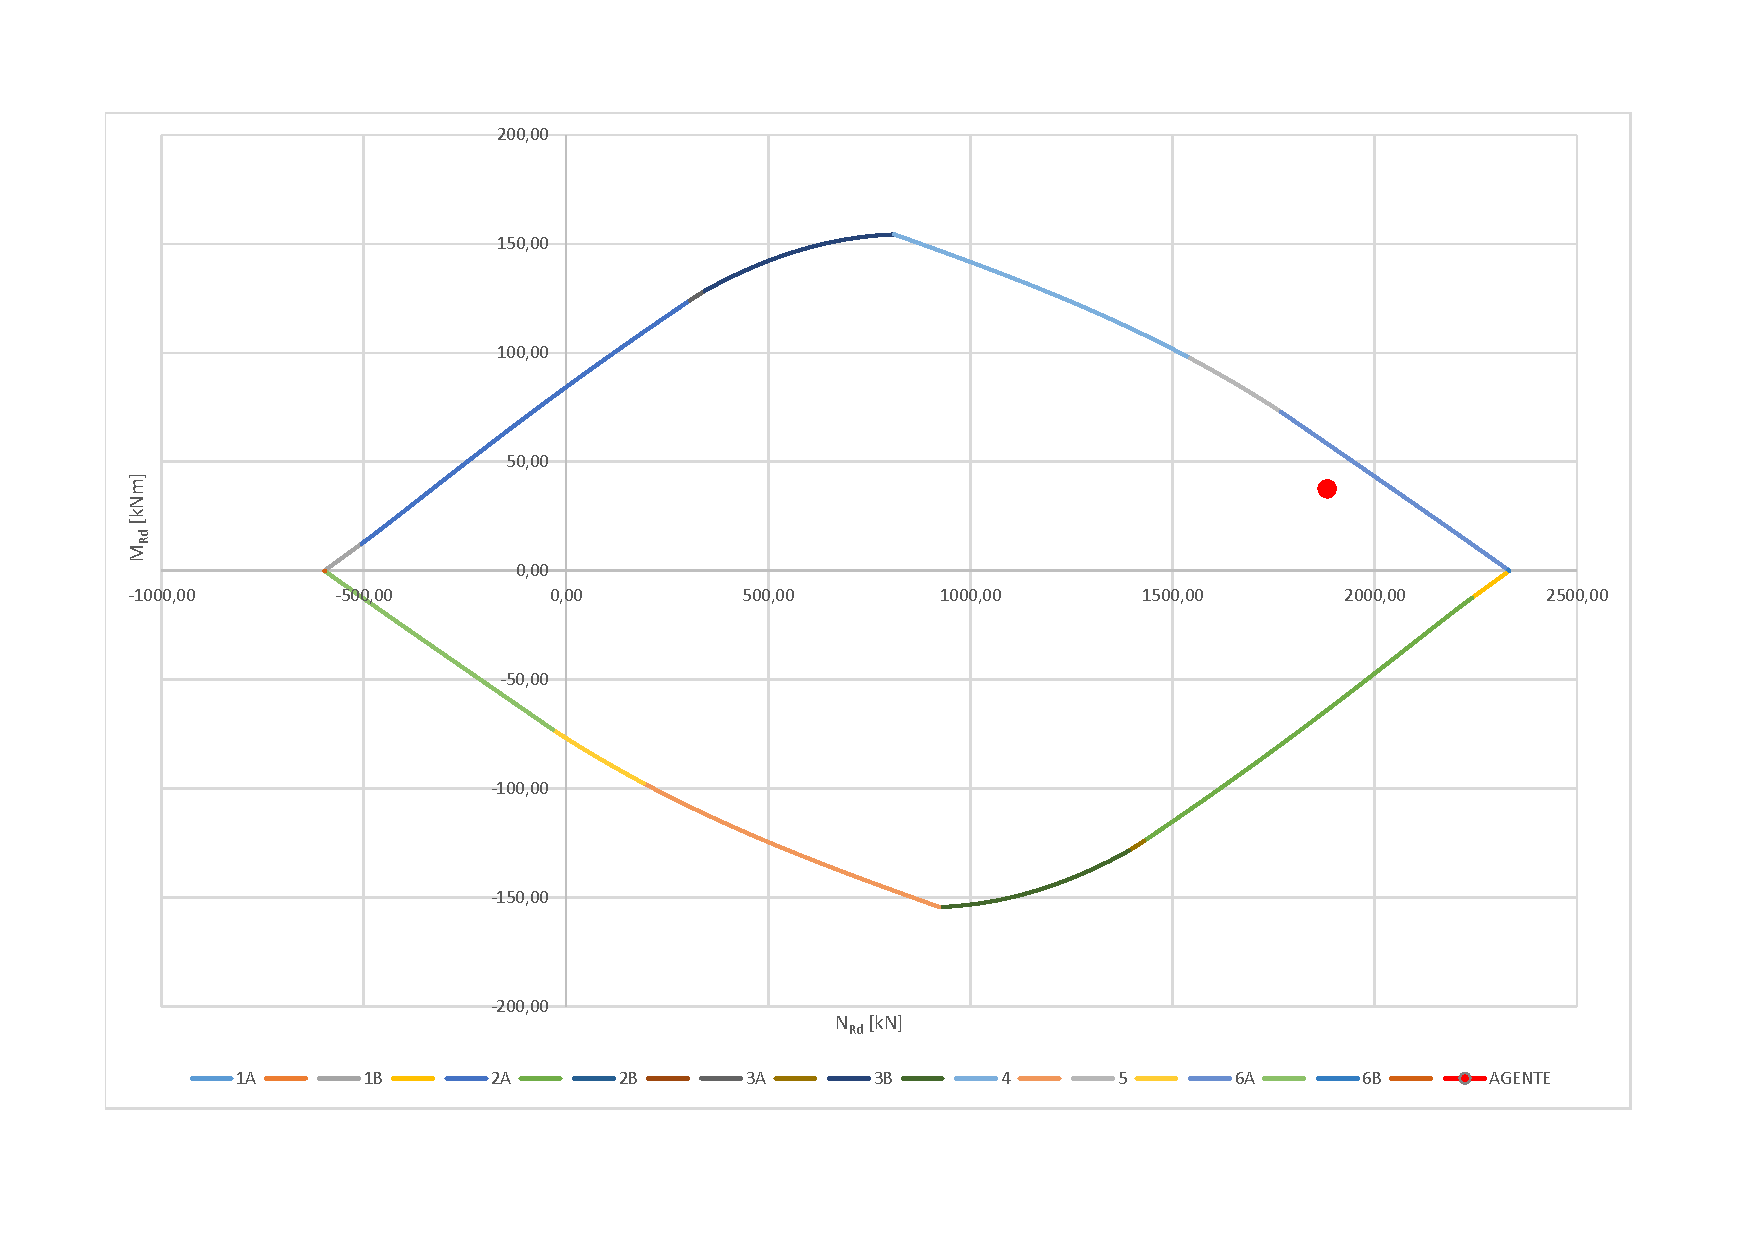
\includegraphics[width=\textwidth]{P27_dominio_M-N}
	\caption{Dominio di resistenza $M-N$ e sollecitazione agente}
\end{figure}

\begin{figure}
    \centering
	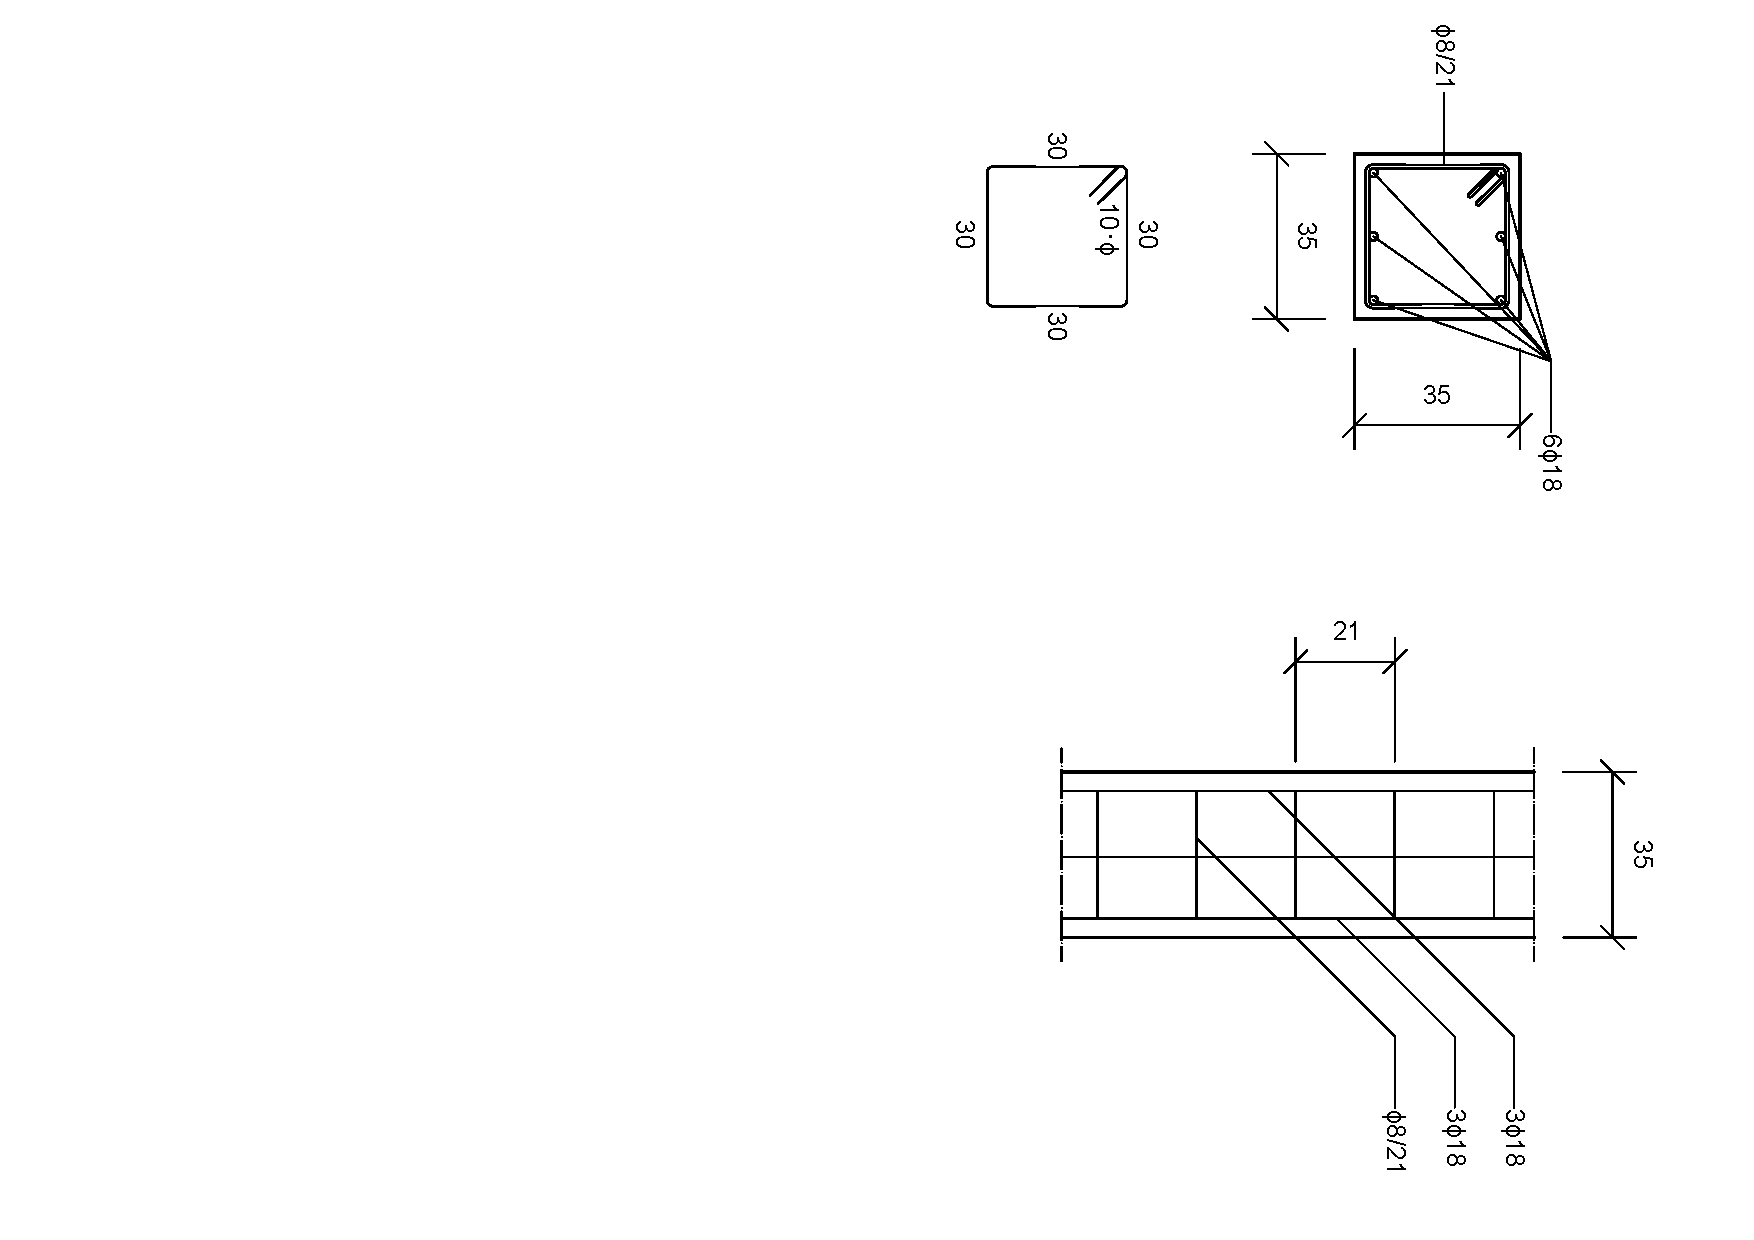
\includegraphics[angle=90, width=\textwidth]{../../disposizioneArmaturePilastro}
	\caption{Disposizione delle armature nel pilastro}
\end{figure}

\section{Verifica di stabilità}
Per elementi snelli quali pilastri, la normativa richiede di effettuare la verifica di stabilità. Questa deve tener conto degli effetti flessionali del secondo ordine (instabilità euleriana), ma anche delle imperfezioni geometriche e meccaniche del materiale, nonché degli effetti dovuti alla viscosità del calcestruzzo. 

\subsection{Snellezza limite}
Seguendo quanto specificato nelle \ntc - essendo queste più severe nel calcolo della  snellezza limite -, per pilastri singoli la verifica di stabilità può essere trascurata se la snellezza $\lambda = \frac{l_0}{i}$ dell'elemento è minore o tuttalpiù uguale alla snellezza limite 
\[
\lambda_{lim} = \dfrac{25}{\sqrt{\nu}} = \dfrac{25}{\sqrt{\dfrac{1882\cdot 10^3\,N}{(350^2\cdot14.17)\,N}}} = 24.01
\]
dove $\nu = \frac{N_{Ed}}{A_c\,f_{cd}}$ è l'azione assiale adimensionalizzata. La snellezza del pilastro, supponendo uno schema statico appoggio - appoggio, è
\[
\lambda = \dfrac{l_0}{i} = \dfrac{l}{\sqrt{\dfrac{J}{A}}} = \dfrac{l}{\sqrt{\dfrac{\dfrac{b^4}{12}}{b^2}}} = \dfrac{l}{\dfrac{b}{\sqrt{12}}} = \dfrac{\sqrt{12}\cdot 3500\,mm}{350\,mm} = 34.641 > \lambda_{lim} = 24.01
\]
dove il raggio giratore di inerzia $i$ è riferito alla sezione in calcestruzzo non fessurata (tutta la sezione).

Poiché $\lambda > \lambda_{lim}$ è necessario eseguire la verifica di stabilità.

\subsection{Verifica di stabilità per elementi isolati}
Per quanto riguarda le verifica di stabilità di elementi isolati la normativa italiana rimanda a documenti di comprovata validità come, ad esempio, l'\ec che - al capitolo \textbf{5.8} descrive i metodi di analisi del secondo ordine. Tra questi è presente il \textit{metodo della curvatura nominale}, basato sul metodo della colonna modello, e il metodo della rigidezza nominale, utilizzabile anche per verifiche su strutture complesse; entrambi sono dei metodi semplificati.

\subsubsection{Metodo della curvatura nominale}
Questo metodo è applicabile a colonne isolate soggette ad azione assiale costante, di sezione e armatura costante lungo tutta l'altezza. Il metodo consiste nel confrontare il momento sollecitante massimo - tenendo conto degli effetti del secondo ordine - con il momento resistente ultimo della sezione fissato lo sforzo assiale e stimando la curvatura. 

L'eccentricità totale è data da
\begin{equation}
	\label{eq:e_tot}
e_{tot} = e_0 + e_\alpha + e_{II}
\end{equation}
dove $e_0=\frac{M_{Ed}}{N_{Ed}}$ è l'eccentricità del primo ordine calcolata precedentemente ($e_0 = 20\,mm$), mentre $e_\alpha$ è l'eccentricità dovuta alle imperfezioni geometriche definita come 
\begin{equation}
    \label{eq:e_alpha}
	e_\alpha = \theta_i\,\dfrac{l_0}{2} = \dfrac{l_0}{400}
\end{equation}
essendo $\theta_i$ l'eccentricità di montaggio assunta pari a $1/_{200}$. Infine $e_{II}$ è l'eccentricità del secondo ordine e - dal \ec - è definita come
\begin{equation}
	\label{eq:e_II}
e_{II} = \dfrac{1}{r}\,\dfrac{l_0^2}{c}
\end{equation}

Il termine $c$ dipende dalla distribuzione della curvatura e può essere assunto pari a $\pi^2 \simeq 10$. La curvatura $1/_r$ è definita nell'equazione \textbf{(5.34)} come
\begin{equation}
    \label{eq:chi_eurocode}
	\dfrac{1}{r} = K_r\,K_\phi\,\dfrac{1}{r_0}
\end{equation}
ove $K_r$ è un fattore di correzione che dipende dall'azione assiale
\begin{align*}
K_r &= \dfrac{n_u-n}{n_u - n_{bal}} \leq 1\\
n &= \dfrac{N_{Ed}}{A_c\,f_{cd}} = 1.084\\
\omega &= \dfrac{A_{s,tot}\,f_{yd}}{A_c\,f_{cd}} = 0.344\\
n_u &= 1+\omega = 1.344\\
n_{bal} &= 0.4
\end{align*}
da cui
\[
    K_r = 0.275 < 1
\]
mentre $K_\phi$ tiene conto degli effetti viscosi del calcestruzzo
\begin{align*}
	K_\phi &= 1 + \beta\,\phi_{ef} \geq 1\\
	\beta &= 0.35 + \dfrac{f_{ck}}{200}  - \dfrac{\lambda}{150} = 0.244
\end{align*}

Il coefficiente di viscosità effettivo è definito dalla \ec come
\[
\phi_{ef}  = \phi(\infty, t_0)\,\dfrac{M_{0Eqp}}{M_{0Ed}}
\]

$M_{0Ed} = N_{Ed}\,e_0 = 1882\,kN\cdot 0.020\,m = 37.64\,kN\,m$ mentre $M_{0Eqp}$ è riferita alla combinazione quasi permanente. L'azione assiale riferita a questa combinazione si può trovare in tabella~\ref{tab:P27_axialLoad_sleQP} di pagina~\pageref{tab:P27_axialLoad_sleQP} e vale $N_{Ed}^{QP} = 1101.30\,kN$; il rispettivo momento vale perciò $M_{0Eqp} = 1101.30\,kN\cdot 0.020\,m = 22.03\,kN\,m$. Il coefficiente di visco a tempo infinito $\phi (\infty, t_0) = 1$ si ricava dalla tabella \textbf{11.2.VI} delle \ntc e supponendo un'umidità relativa del $75\%$, un tempo di applicazione dei carichi quasi permanente $t_0 \geq 60\,giorni$ e quindi interpolando i valori della tabella richiamata poco sopra si ottiene 
\[
\phi(\infty, t_0; h_0 = 350\,mm) = 1.683
\]
da cui
\[
\phi_{ef} = 1.863\cdot\dfrac{22.03}{37.64} = 1.09 
\]
e sostituendo
\[
    K_\phi = 1+ 0.244\cdot 1.09 = 1.27 > 1
\]

Infine
\[
\dfrac{1}{r_0} = \dfrac{\epsilon_{yd}}{0.45\,d} = \dfrac{\dfrac{f_{yd}}{E_s}}{0.45\,d} = \dfrac{1.863\cdot 10^{-3}}{0.45\cdot 310\,mm} = 1.3355\cdot 10^{-5}\,\dfrac{1}{mm}
\]
dove $\epsilon_{yd}$ è la deformazione a snervamento dell'acciaio. In definitiva, sostituendo i valori numerici nella \eqref{eq:chi_eurocode} si ottiene
\begin{equation}
    \label{eq:chi_value}
	\dfrac{1}{r} = 0.275\cdot 1.14\cdot 1.3355\cdot 10^{-5}\,\dfrac{1}{mm} = 4.6642\cdot 10^{-6}\,\dfrac{1}{mm}
\end{equation}

Supponendo uno schema statico tale per cui $l_0 = l = 3500\,mm$ le \eqref{eq:e_II} e \eqref{eq:e_alpha} diventano rispettivamente
\begin{align*}
	e_{II} &= 4.6642\cdot 10^{-6}\,\dfrac{1}{mm}\cdot \dfrac{3500^2\,mm^2}{10} = 5.71\,mm\\
	e_\alpha &= \dfrac{3500\,mm}{400} = 8.75\,mm
\end{align*}

L'eccentricità totale è
\[
e_{tot} = 20\,mm + 8.75\,mm + 5.71\,mm = 34.46\,mm
\]
\noindent
Il momento di progetto alla base del pilastro - tenendo conto degli effetti del secondo ordine - è
\begin{equation}
    \label{eq:MEd_secondo_ordine}
	M_{Ed} = N_{Ed} \cdot e_{tot} = 1882\,kN\cdot 34.46\cdot 10^{-3}\,m = 64.85\,kN\,m
\end{equation}

Come si può vedere nel diagramma M -- N di figura~\ref{fig:P27_dominio_M-N_stabilita} la sezione non è verificata.
\begin{figure}
    \centering
	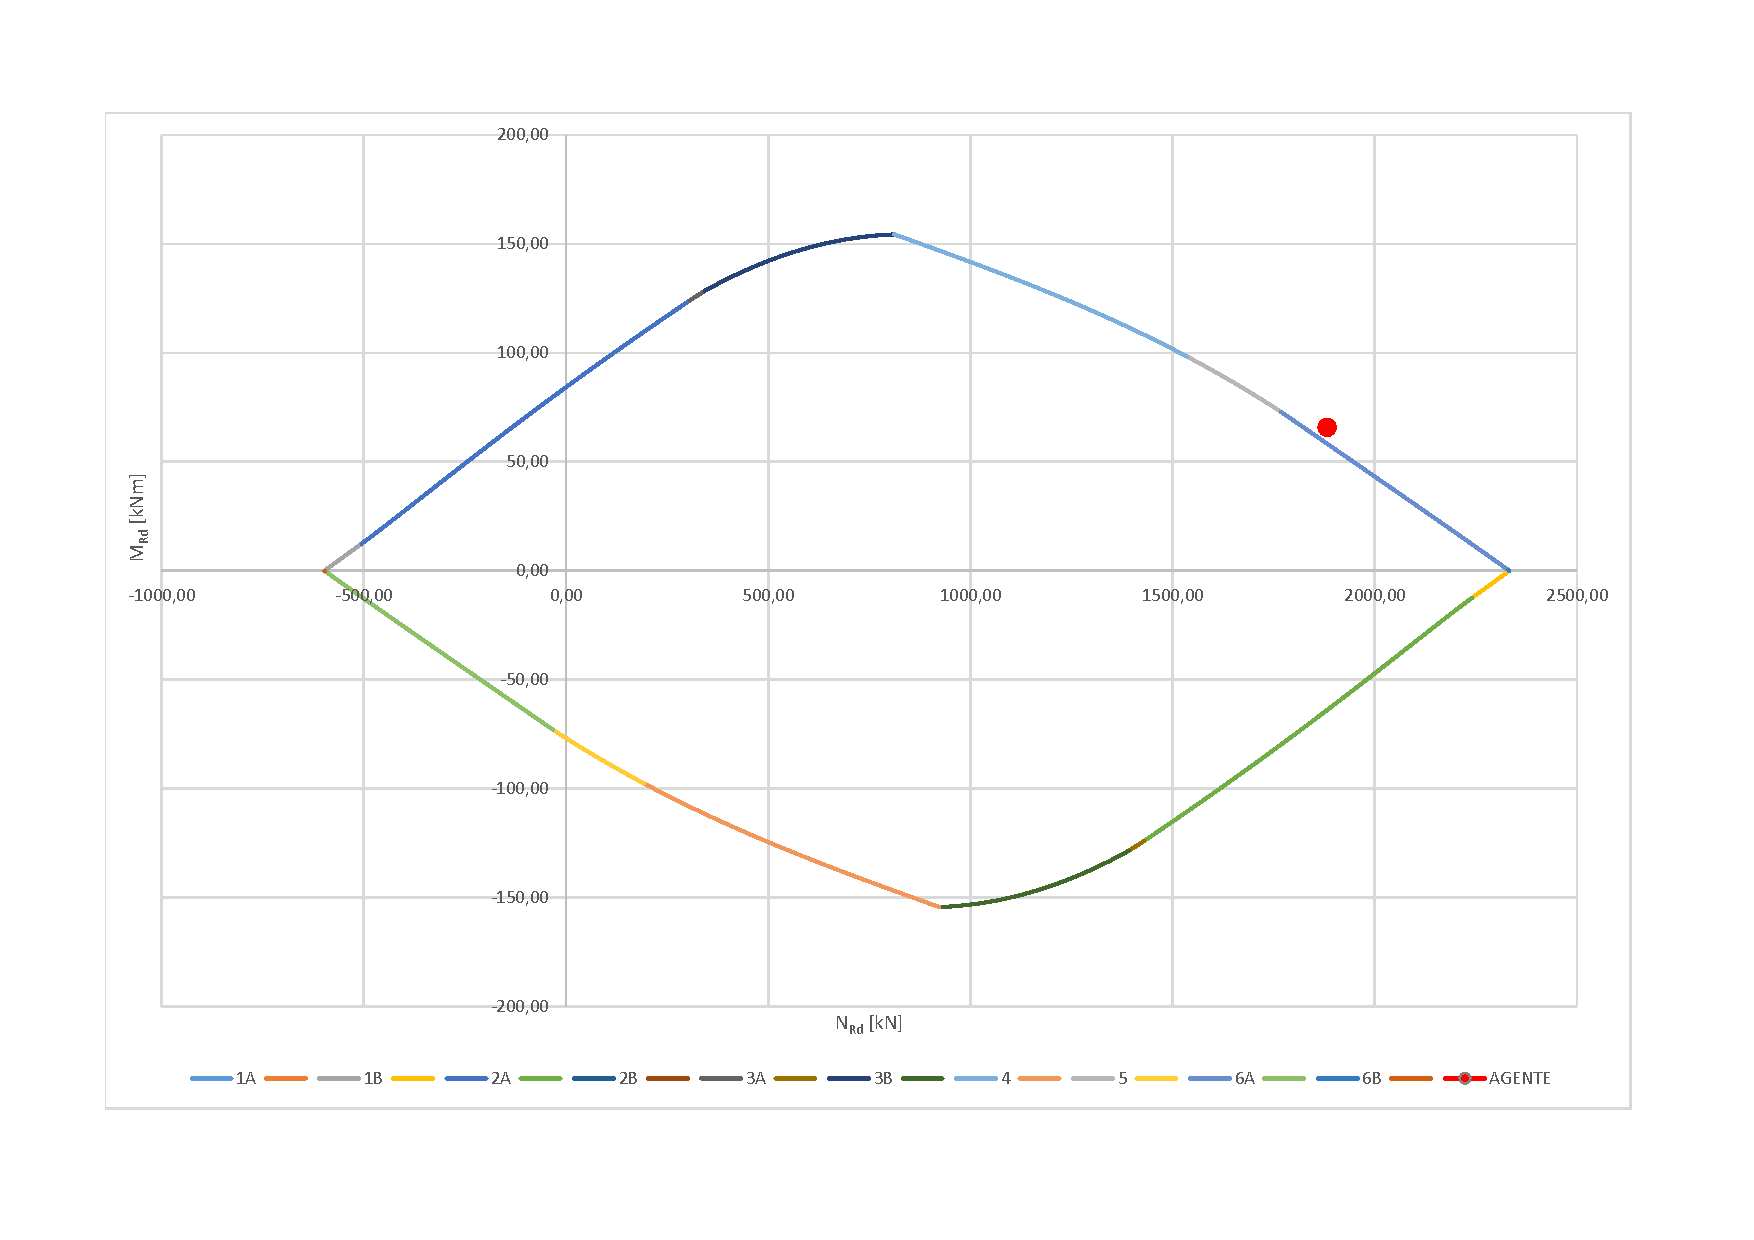
\includegraphics[width=\textwidth]{P27_dominio_M-N_stabilita}
	\caption{Dominio M -- N con gli effetti del secondo ordine}
	\label{fig:P27_dominio_M-N_stabilita}
\end{figure}


Utilizzando come armatura
\begin{align*}
    A_s &= 3\,\Phi\,20\,mm = 300\,\pi\,mm^2 = 942.48\,mm^2\\
	A'_s &= 3\,\Phi\,20\,mm = 300\,\pi\,mm^2 = 942.48\,mm^2\\
	\Phi_{st} &= 8\,mm\\
	s &= 240\,mm\\
\end{align*}
si ottengono i seguenti valori
\begin{align*}
	N_{Rd} &= 0.8\cdot A_c\,f_{cd} + A_{s,tot}\,f_{yd} = 2126.24\,kN > N_{Ed} = 1882\,kN\\
	\omega &= \dfrac{A_{s,tot}\,f_{yd}}{A_c\,f_{cd}} = 0.425\\
	n_u &= 1+\omega = 1.425\\
	K_r &= 0.333\\
	K_\phi &= 1.27\\
	\dfrac{1}{r} &= 5.648\cdot 10^{-6}\,\dfrac{1}{mm}\\
	e_{II} &= 6.92\,mm\\
	e_{tot} &= 35.67\,mm\\
	M_{Ed} &= 1882\,kN \cdot 35.67\cdot 10^{-3}\,m = 67.13\,kN\,m
\end{align*}

Come rappresentato in figura~\ref{fig:P27_dominio_M-N_stabilita_corretto} con questa configurazione la sezione risulta verificata ad instabilità con il metodo della curvatura nominale.

\begin{figure}
	\centering
	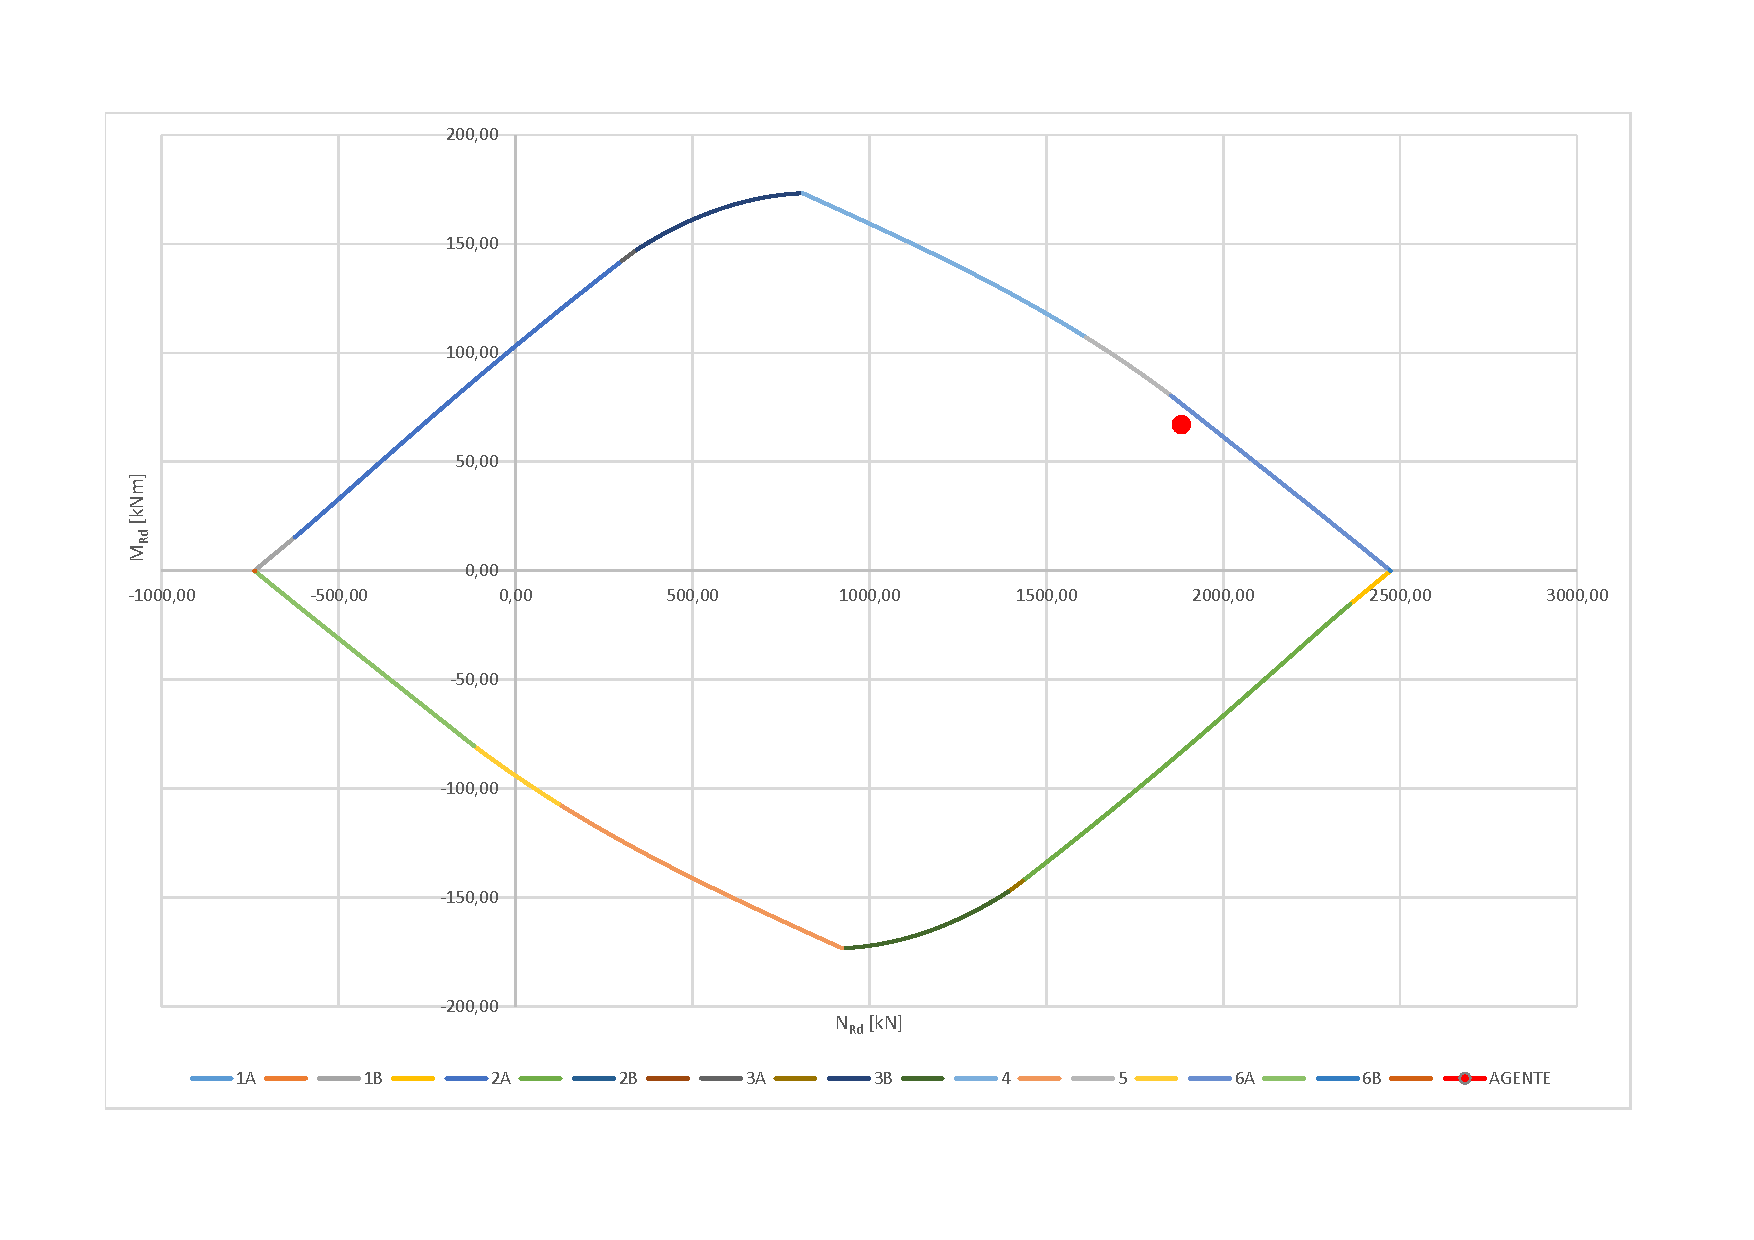
\includegraphics[width=\textwidth]{P27_dominio_M-N_stabilita_corretto}
	\caption{Dominio M -- N con gli effetti del secondo ordine con armatura $6\,\Phi\,20$}
	\label{fig:P27_dominio_M-N_stabilita_corretto}
\end{figure}

\subsubsection{Metodo della rigidezza nominale}
Il metodo della rigidezza nominale consiste nell'analisi non lineare di tipo geometrico ed è applicabile ad elementi di strutture di sezione qualunque; decade, quindi, l'obbligo di avere una sezione costante lungo tutto lo sviluppo dell'elemento che era presente nel metodo della curvatura nominale. 

Questo si basa sulla stima delle rigidezza flessionali che secondo l'\ec si possono disaccoppiare e riscrivere come
\begin{equation}
    \label{eq:EI_eurocode}
	E\,I = K_c\,E_{cd}\,I_c + K_s\,E_s\,I_s
\end{equation}

Come anticipato le rigidezze dei materiali sono disaccoppiate. La rigidezza finale è data da un'aliquota riferita al calcestruzzo modulata dal coefficiente $K_c$ che tiene conto di tutti gli effetti di viscosità, fessurazione, etc. del materiale. Il rapporto geometrico di armatura (totale) è di
\[
\rho = \dfrac{A_s + A'_s}{A_c} = 0.0154
\]

Si assume
\begin{align*}
    K_s &= 1\\
	I_s &= A_s\,\left(d-\dfrac{h}{2}\right) + A'_s\,\left(\dfrac{h}{2}-d''\right) = 254469\,mm^4\\
	E_s &= 210000\,MPa\\
	k_1 &= \sqrt{\dfrac{f_{ck}}{20}} = 1.12\\
	k_2 &= \min\left\{\dfrac{N_{Ed}}{A_c\,f_{cd}}\,\dfrac{\lambda}{170}; 0.20\right\} = \min\{0.22; 0.20\} = 0.20\\ 
	K_c &= \dfrac{k_1\,k_2}{1+\,\phi_{ef}} = \dfrac{1.12\cdot0.20}{1+1.09} = 0.107\\
	E_{cd} &= \dfrac{E_{cm}}{\gamma_{CE}} = \dfrac{31476\,MPa}{1.2} = 26230\,MPa\\
	I_c &= \dfrac{b\,h^3}{12} = 1.25052\cdot 10^9\,mm^4\\
\end{align*}

Dal \textbf{NAD} si ha che $\gamma_{CE} = 1.2$.
La rigidezza stimata vale
\[
E\,I = 0.107\cdot 26230\,MPa\cdot 1.25052\cdot 10^9\,mm^4 + 1\cdot210000\,MPa\cdot254469\,mm^4 = 3.56\cdot 10^{12} N\,mm^2 
\]

L'amplificazione dei momenti è data da
\begin{equation}
    \label{eq:amplificazione_momenti}
	M_{Ed} = M_{0Ed}\,\left[1 + \dfrac{\beta}{\dfrac{N_B}{N_{Ed}}-1}\right]
\end{equation}
dove 
\[ M_{0Ed} = 1882\,kN\cdot (20+8.75)\cdot 10^{-3}\,m = 54.11\,kN\,m\]
mentre $\beta=\frac{\pi^2}{c_0} = \frac{\pi^2}{8} = 1.234$ ($c_0=8$ per distribuzioni di momento costanti) e $N_B$ è il carico critico euleriano calcolato con la rigidezza nominale
\[
N_B = \dfrac{E\,I\,\pi^2}{l_0^2} = \dfrac{3.56\cdot 10^{12} N\,mm^2\,\pi^2}{3500^2\,mm^2} = 2868.23\,kN
\]

Sostituendo
\[
M_{Ed} = 54.11\,kN\,m\,\left[1+\dfrac{1.234}{\dfrac{2868.23\,kN}{1882\,kN}-1}\right] = 181.53\,kN\,m
\]

Con la configurazione scelta sulla base del metodo della curvatura nominale ($6\,\Phi\,20\,mm$) la sezione non è verificata per la stabilità. Perché la sezioni superi la verifica sarebbe necessario inserire $12\,\Phi\,22\,mm$ divisi tra il lato superiore e il lato inferiore in maniera simmetrica. La differenza con il metodo precedentemente esposto è sostanziosa (il momento agente è quasi triplicato) (si veda la figura~\ref{fig:diagramma_M-N_rigidezzaNominale}).
 
\begin{figure}
    \centering
	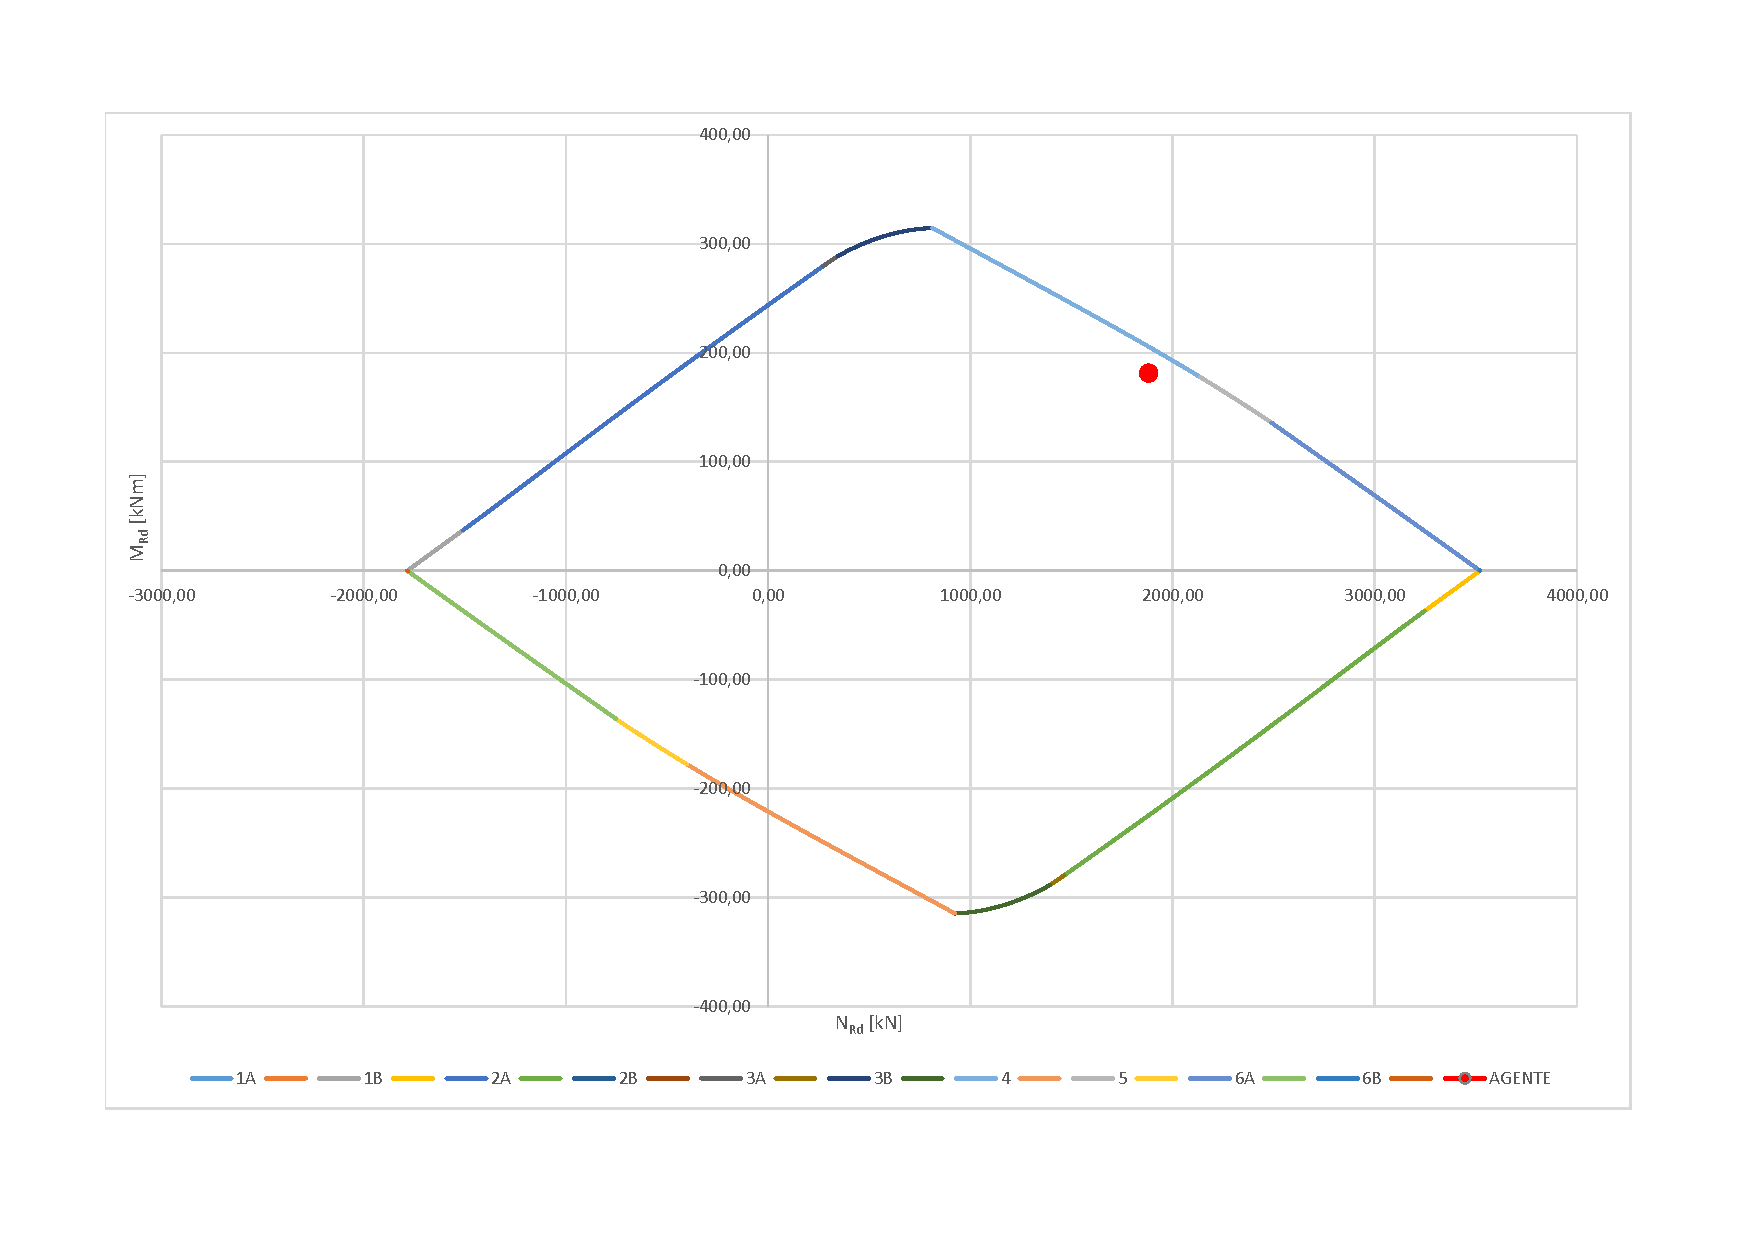
\includegraphics[width=\textwidth]{P27_dominio_M-N_stabilita_rigidezzaNominale}
	\caption{Diagramma $M-N$ -- metodo della rigidezza nominale con $12\,\Phi\,22\,mm$}
	\label{fig:diagramma_M-N_rigidezzaNominale}
\end{figure}

Considerando un copriferro $c = 25\,mm$ la base minima necessaria è
\[
b_{min} = 2\,c + n_b\,\Phi_{st} + n\, \Phi_l + (n-1)\,i = (2\cdot 25 + 2\cdot 8 + 6\cdot 22 + 5\cdot 25)\,mm = 323\,mm < b = 350\,mm
\]

Considerando il modello più sfavorevole, la sezione di progetto ha le seguenti caratteristiche
\begin{align*}
    b &= 350\,mm\\
	h &= 350\,mm\\
	A_s &= 6\,\Phi\,22\,mm\\
	A'_s &= 6\,\Phi\,22\,mm\\
	A_{s,tot} &= 12\,\Phi\,22\,mm = 4561.60\,mm^2 < A_{s,max} = 4900\,mm^2\\
	s_{max} &= \min\{12\,\Phi_{l,min}; 250\,mm\} = \min\{264\,mm; 250\,mm\} = 250\,mm \\
	s &= 250\,mm\\
	\Phi_{st,min} &= \max\left\{\dfrac{\Phi_{l,max}}{4}; 6\,mm\right\} = \max\{5.5\,mm; 6\,mm\} = 6\,mm\\
	\Phi_{st}&=  8\,mm
\end{align*}

\begin{figure}
	\centering
	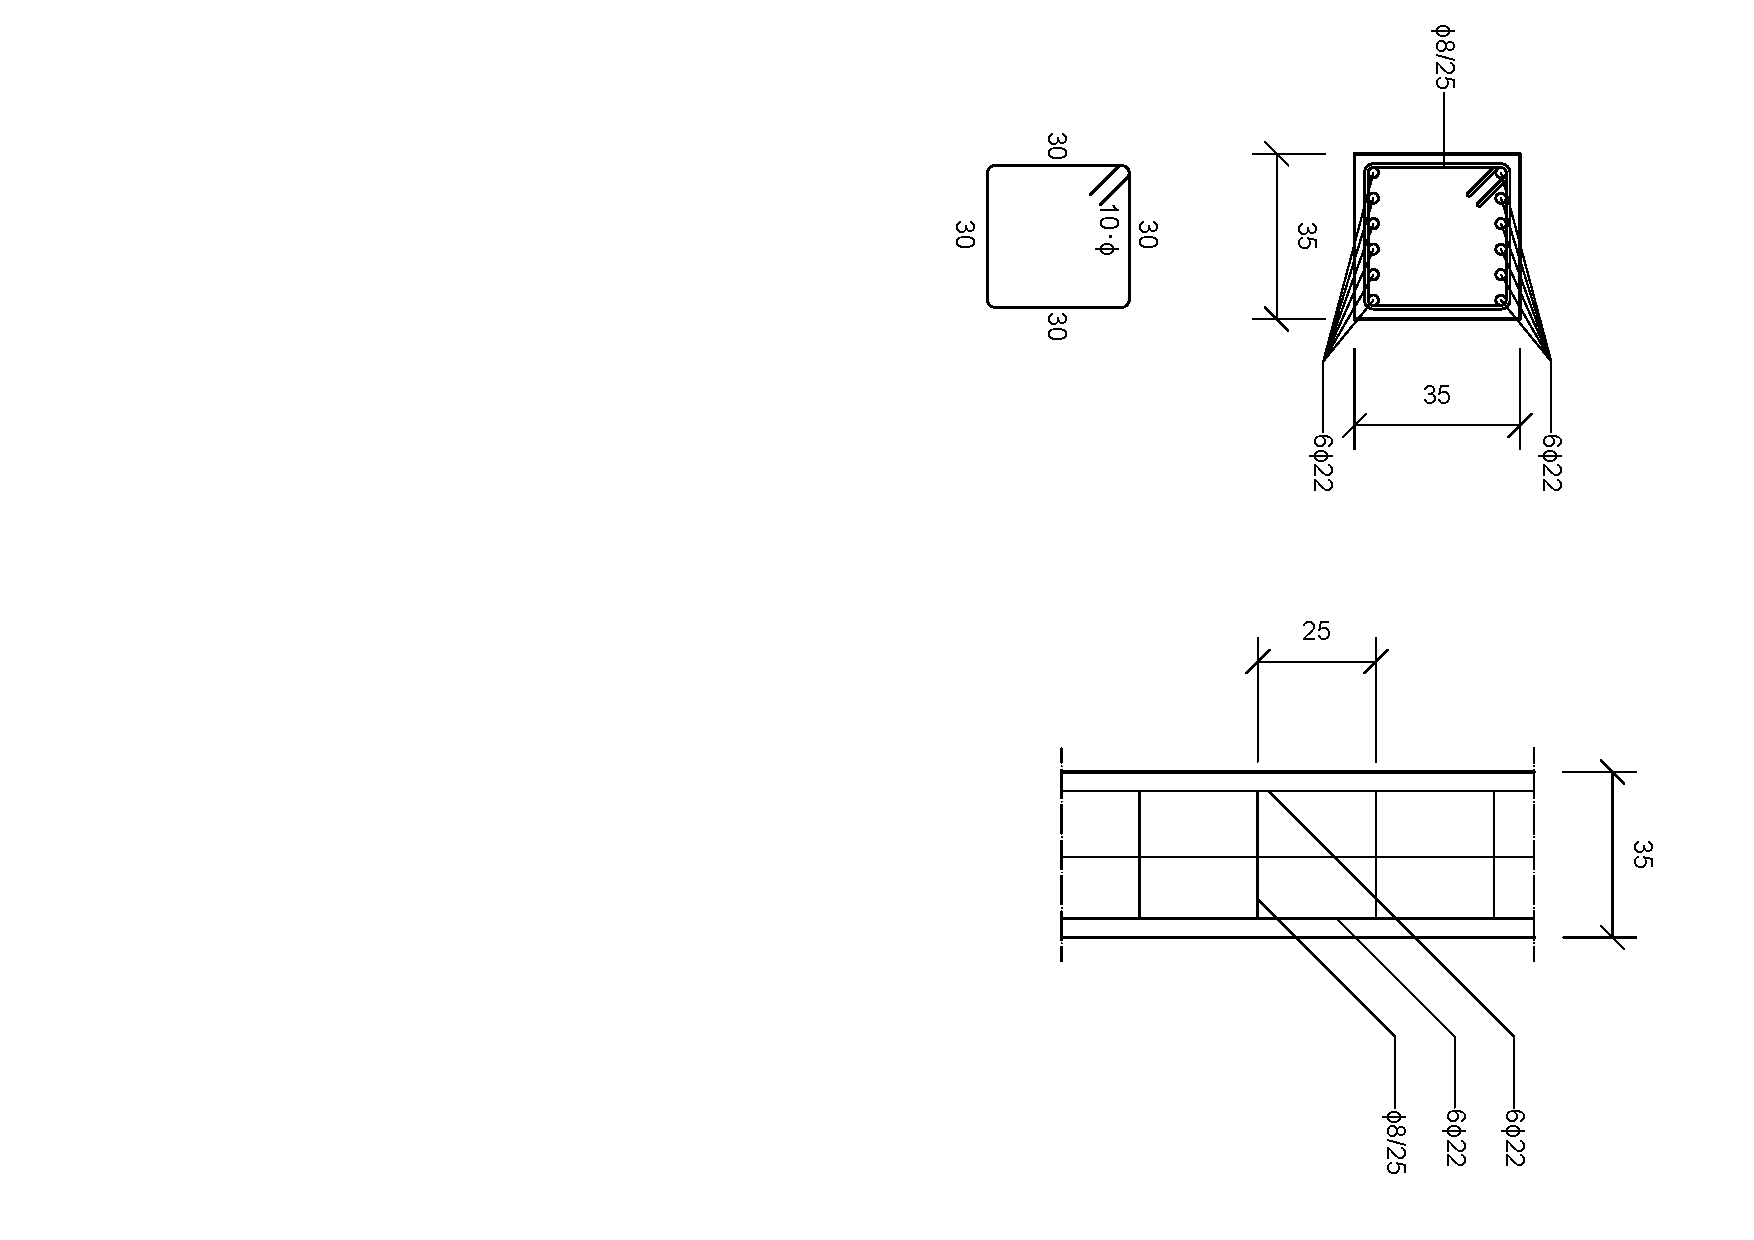
\includegraphics[angle=90, width=\textwidth]{../../disposizioneArmaturePilastro_stabilita}
	\caption{Disposizione delle armature nel pilastro dopo l'analisi di stabilità}
	\label{fig:disposizioneArmaturePilastroFinali}
\end{figure}
\cleardoublepage
\subsubsection{Metodo della colonna modello}
Come ulteriore verifica si tratta il metodo della colonna modello, su cui è basato il metodo della curvatura nominale. Il modello consiste nel verificare l'intersezione tra i momenti di primo e secondo ordine con l'andamento del diagramma momento curvatura ($M-\chi$) della sezione di figura~\ref{fig:disposizioneArmaturePilastroFinali}. Il diagramma $M-\chi$ (o $M-\frac{1}{r}$) può essere semplificato calcolando tre punti significativi:
\begin{itemize}
    \item il punto di \emph{prima fessurazione};
    \item il punto di \emph{snervamento delle armature} (inferiori o superiori);
    \item il punto di \emph{collasso}.
\end{itemize}

Ogni punto è descritto da una coppia $(\chi, M)$. Nelle righe seguenti verranno espressi i calcoli per $N_{Ed} = 1882\,kN$.

\subsubsection*{Prima fessurazione}

Prima della fessurazione del calcestruzzo la sezione resistente comprende sia il calcestruzzo compresso che quello teso, in aggiunta alle armature. La fessurazione del calcestruzzo avviene per una deformazione fissata dal \emph{Model Code} di
\[
\epsilon_{ctu} = 0.3\,\permil
\]

In questa configurazione, applicando la linearità del diagramma delle deformazioni, si possono calcolare le deformazioni delle fibre significative in funzione della posizione dell'asse neutro 
\begin{align*}
	\epsilon_c^s &= \dfrac{\epsilon_{ctu}}{h-x}\,x\\
	\epsilon_s &= \dfrac{\epsilon_{ctu}}{h-x}\,(d-x)\\
	\epsilon'_s &= \dfrac{\epsilon_{ctu}}{h-x}\,(x-d'')
\end{align*}
dove $x$ è un'incognita del problema e si calcola dall'equilibrio alla traslazione
\[
C_c + C_s - T_s - T_c = N_{Ed}
\]

Si applica l'ipotesi di parabola rettangolo non completamente sviluppato, con $\epsilon_c^s > \epsilon_{c2}$ con armature superiori compresse, armature inferiori tese ed entrambe in campo elastico; perciò
\begin{align*}
&b\,\int_0^{x_0(x)} f_{cd}\,\left(1-\left(1-\dfrac{\epsilon_{ctu}}{\epsilon_{c2}}\,\dfrac{y}{h-x}\right)^2\right)\,dy + b\,f_{cd}\,\left(x-x_0(x)\right) + A'_s\,E_s\,\epsilon'_s(x)+\\ 
&- A_s\,E_s\,\epsilon_s (x) - b\,f_{ctd}\,\dfrac{2}{3}\,(h-x) = N_{Ed}
\end{align*}
dove
\[
x_0 (x) = \dfrac{\epsilon_c^s}{\epsilon_{c2}}\,x
\]

Risolvendo risulta 
\[ x_1 = 306.114\,mm\]

Il controllo sulle deformazioni
\begin{align*}
	\epsilon_c^s &= 2.09\,\permil = \epsilon_{c2}\\
	\epsilon_s &= 0.0265\,\permil < \epsilon_{se}\\
	\epsilon'_s &= 1.819\,\permil < \epsilon_{se}
\end{align*}

Inoltre
\begin{align*}
	\lambda &= \dfrac{1}{x}\,\dfrac{b\,\bigints_0^{x_0(x)} f_{cd}\,\left(1-\left(1-\dfrac{\epsilon_{ctu}}{\epsilon_{c2}}\,\dfrac{y}{h-x}\right)^2\right)\,(x-y)\,dy + b\,\bigint_{x_0(x)}^x f_{cd}\,(x-y)\,dy}{b\,\bigints_0^x f_{cd}\,\left(1-\left(1-\dfrac{\epsilon_{ctu}}{\epsilon_{c2}}\,\dfrac{y}{h-x}\right)^2\right)\,dy + b\,f_{cd}\,(x-x_0(x))} = 0.37332\\
	\psi =& \dfrac{C_c}{b\,x\,f_{cd}} = \dfrac{b\,\bigints_0^{x_0(x)} f_{cd}\,\left(1-\left(1-\dfrac{\epsilon_{ctu}}{\epsilon_{c2}}\,\dfrac{y}{h-x}\right)^2\right)\,dy + b\,f_{cd}\,(x-x_0(x))}{b\,x\,f_{cd}} = 0.67116
\end{align*}

La coppia curvatura -- momento relativa è
\begin{align}
	\chi_1 &= \dfrac{\epsilon_{c}^s (x_1) - \epsilon_s (x_1)}{d} = 6.66448\cdot 10^{-3}\,\dfrac{1}{m}\\
	\small M_1 &= C_c\,\left(\dfrac{h}{2} - \lambda\,x_1	\right) + C_s\,\left(\dfrac{h}{2}-d''\right) + T_s\,\left(d-\dfrac{h}{2}\right) + T_c\,\left(\dfrac{h}{6}+\dfrac{x_1}{3}\right) = 182.277\,kN\,m
\end{align}

\subsubsection*{Snervamento armature}
La sezione è già fessurata, perciò il calcestruzzo teso non dà alcun contributo. Si ipotizza che le armature snervate siano quelle superiori
\begin{align*}
\epsilon'_s &= \epsilon_{se} = 1.863\,\permil\\
\epsilon_c^s &= \dfrac{\epsilon'_s}{x-d''}\,x\\
\epsilon_s &= \dfrac{\epsilon'_s}{x-d''}\,(d-x)\\
\end{align*}

Si considerano le armature inferiori in campo elastico e il calcestruzzo tale per cui $\epsilon_c^s > \epsilon_{c2}$
\[
b\,\int_0^{x_0(x)} f_{cd}\,\left(1-\left(1-\dfrac{\epsilon_c^s (x)}{\epsilon_{c2}}\,\dfrac{y}{x}\right)^2\right)\,dy + b\,f_{cd}\,\left(x-x_0(x)\right) + A'_s\,f_{yd} - A_s\,E_s\,\epsilon_s(x) = N_{Ed}
\]
dove
\[
x_0(x) = \dfrac{\epsilon_{c2}}{\epsilon_c^s (x)}\,x 	
\]

Si ricava
\[
    x_2 = 277.23\,mm
\]
mentre le deformazioni
\begin{align*}
    \epsilon_c^s &= 2.18\,\permil\\
	\epsilon_s &= 0.257\,\permil
\end{align*}
che sono compatibili con le ipotesi effettuate. Inoltre
\begin{align*}
    \lambda &= 0.3807\\
	\psi &= 0.694
\end{align*}

I valori di curvatura e momento sono
\begin{align}
	\chi_2 &= 7.855\cdot 10^{-3}\,\dfrac{1}{m}\\
	M_2 &= 203.38\,kN\,m
\end{align}

\subsubsection*{Collasso}
In condizioni di collasso si assume
\[
\epsilon_c^s = \epsilon_{cu}
\]
con armature inferiori in campo elastico e armature superiori snervate.

\[
b\,\int_0^{x_0(x)} f_{cd}\,\left(1-\left(1-\dfrac{\epsilon_{cu}}{\epsilon_{c2}}\,\dfrac{y}{x}\right)^2\right)\,dy + b\,f_{cd}\,\left(x-x_0(x)\right) + A'_s\,f_{yd} - A_s\,E_s\,\epsilon_s(x) = N_{Ed}
\]
da cui
\[
    x_3 = 284.29\,mm
\]
mentre le deformazioni
\begin{align*}
	\epsilon_s &= 0.3165\,\permil\ < \epsilon_{se}\\
	\epsilon'_s &= 3.01\,\permil > \epsilon_{se}
\end{align*}

I valori di $\lambda$ e $\psi$ sono quelli per il calcestruzzo a collasso
\begin{align*}
    \lambda = 0.415966\\
	\psi = 0.809524
\end{align*}

La terna di valori è
\begin{align}
	\chi_3 &= 10.2693\cdot 10^{-3}\,\dfrac{1}{m}\\
	M_3 &= 205.70\,kN\,m
\end{align}

\begin{figure}
    \centering
	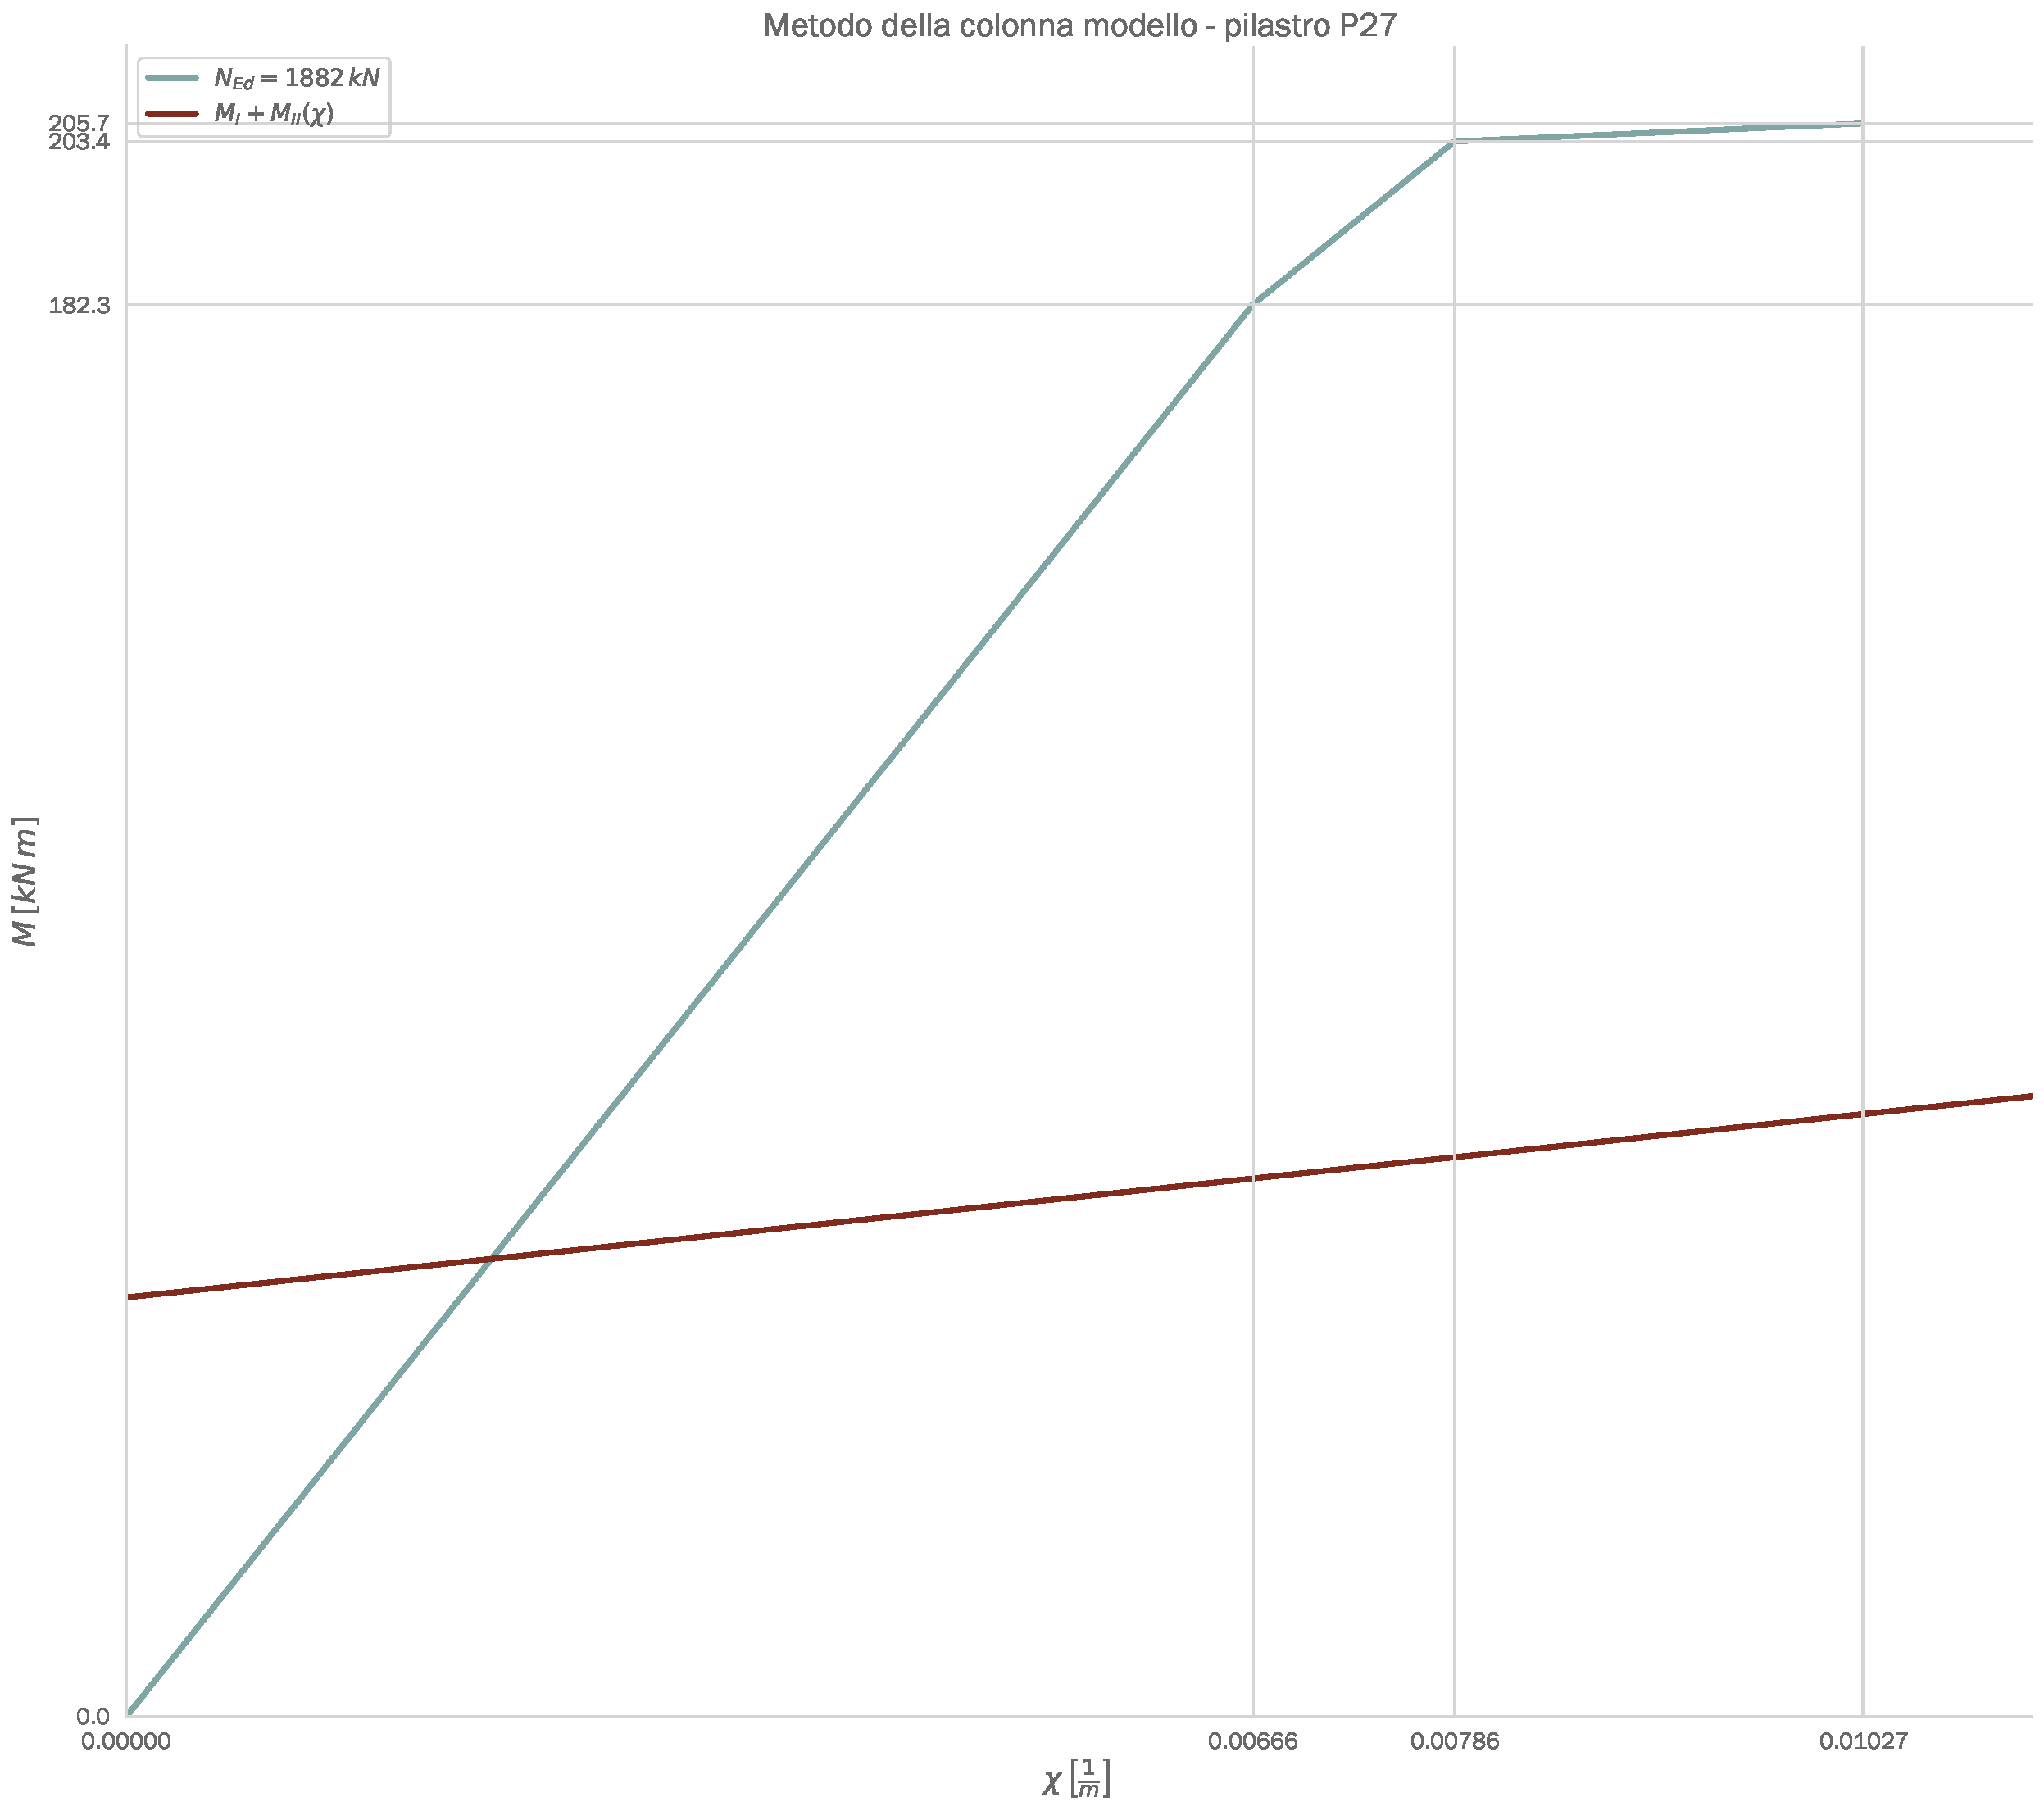
\includegraphics[width=\textwidth]{colonnaModello}
	\caption{Metodo della colonna modello per $N_{Ed} = 1882\,kN$}
	\label{fig:colonnaModello}
\end{figure}

Congiungendo i tre punti risulta la trilatera di figura~\ref{fig:colonnaModello}. L'equazione della retta è tale per cui
\begin{align*}
	M_I + M_{II} (\chi) &= N_{Ed}\,(e_0 + e_\alpha) + N_{Ed}\,\dfrac{1}{r}\,\dfrac{l_0^2}{10} = 1882\,kN \left(28.75\cdot 10^{-3}\,m + 1.225\,m^2\cdot \dfrac{1}{r}\right)\\
	&= 54.11\,kN\,m + 2305.45\,kN\,m^2\cdot \dfrac{1}{r} = 54.11\,kN\,m + 2305.45\,kN\,m^2\cdot \chi
\end{align*}
dove $\frac{1}{r} = \chi$, con $r$ in metri.

Dalla figura~\ref{fig:colonnaModello} si deduce che la sezione non è fessurata per i valori di momento del secondo ordine agenti; si verifica inoltre la stabilità, poiché aumentando l'azione assiale - e perciò la curvatura - l'elemento tende a riportarla a valori di curvatura inferiori.

Si conclude così il progetto del pilastro, che è stato verificato sia agli SLU che all'instabilità.
\cleardoublepage
